\section{Problem 1 – Linear Algebra}

\paragraph{Question 1}
Let $A\in R^{n\times n}$ such that $A = A^T$ and $Ax = \lambda x$ for some eigenvector $x$ and corresponding eigenvalue $\lambda$.
Suppose that $\lambda \in \mathbb{C}$, i.e. $\lambda = a + ib$ for some $a,b\in\mathbb{R}$.
Let's start with $Ax = \lambda x$:
\begin{align*}
    Ax &= \lambda x && \text{take conjugate transpose} \\
    x^H A^H &= \lambda^H x^H && \text{$A$ is real, so $A=A^H$} \\
    x^H A &= \lambda^H x^H && \text{multiply by  $x$} \\
    x^H A x &= \lambda^H x^H x && \text{now,  $Ax = \lambda x$} \\
    \lambda x^H x &= \lambda^H x^H x  \\
    \lambda &= \lambda^H \\
    a + bi &= a - bi
\end{align*}
Hence, Im$(\lambda)$ = 0, which means $\lambda \in R$.


\paragraph{Question 2}
Start with the first eigenpair:
\begin{align*}
    Ax_1 &= \lambda_1 x_1   && \text{take transpose. $A = A^T$} \\
    x_1^T A &= \lambda_1 x_1^T && \text{multiply by $x_2$} \\
     x_1^T A x_2 &= \lambda_1 x_1^T x_2 &&  \\
\end{align*}
Now fiddle with the second eigenpair:
\begin{align*}
    Ax_2 &= \lambda_2 x_2   && \text{left-multiply by $x_1^T$} \\
    x_1^T Ax_2 &= \lambda_2 x_1^T x_2 
\end{align*}
If we subtract both result, we get:
\begin{align*}
    0 = (\lambda_1 - \lambda_2) x_1^T x_2
\end{align*}
Since $\lambda_1 \neq \lambda_2$, then $ x_1^T x_2 = 0$.
In other words, $x_1 \cdot x_2 =0$.

\paragraph{Question 3 - s e n d h e l p}
\begin{equation*}
    A =
\begin{pmatrix}
x & a_1 & b_1 & c_1 \\
x & a_2 & b_2 & c_2 \\
x & a_3 & b_3 & c_3 \\
1 & 1 & 1 & 1
\end{pmatrix}
\end{equation*}
\begin{equation*}
    f(x,y,z) = \text{det}(A)
\end{equation*}

This seems to be difficult. 
I succeeded in computing determinant using Laplace expansion wrt first column, but it gets hardcore later. Any ideas?

\paragraph{Question 4}
Give 3 points that lie on plane $f(x,y,z) = 0$.
When is determinant $=0$? 
For example, when some columns are dependent.
Let's make some columns dependent.
Zum Beispiel, let's take:
\begin{align*}
    x = a_1 && y = a_2 && z = a_3
\end{align*}
Now first and second column are dependent, so $\text{det}(A) = f(x,y,z) = 0$.
To get two others solutions, take $x = b_1, y = b_2, z = b_3$ and $x = c_1, y = c_2, z = c_3$ or simply multiply the first solution by some constants.


\section{Problem 2 – Automata Theory}

\paragraph{Question 1}
\begin{verbatim}
-> O --a--> O --b--> O --b--> (o)
      / \
      \ /
      a,b
\end{verbatim}

\paragraph{Question 2}
See Fig.\ref{fig:w15-2}.
\begin{figure}[!h]
    \centering
    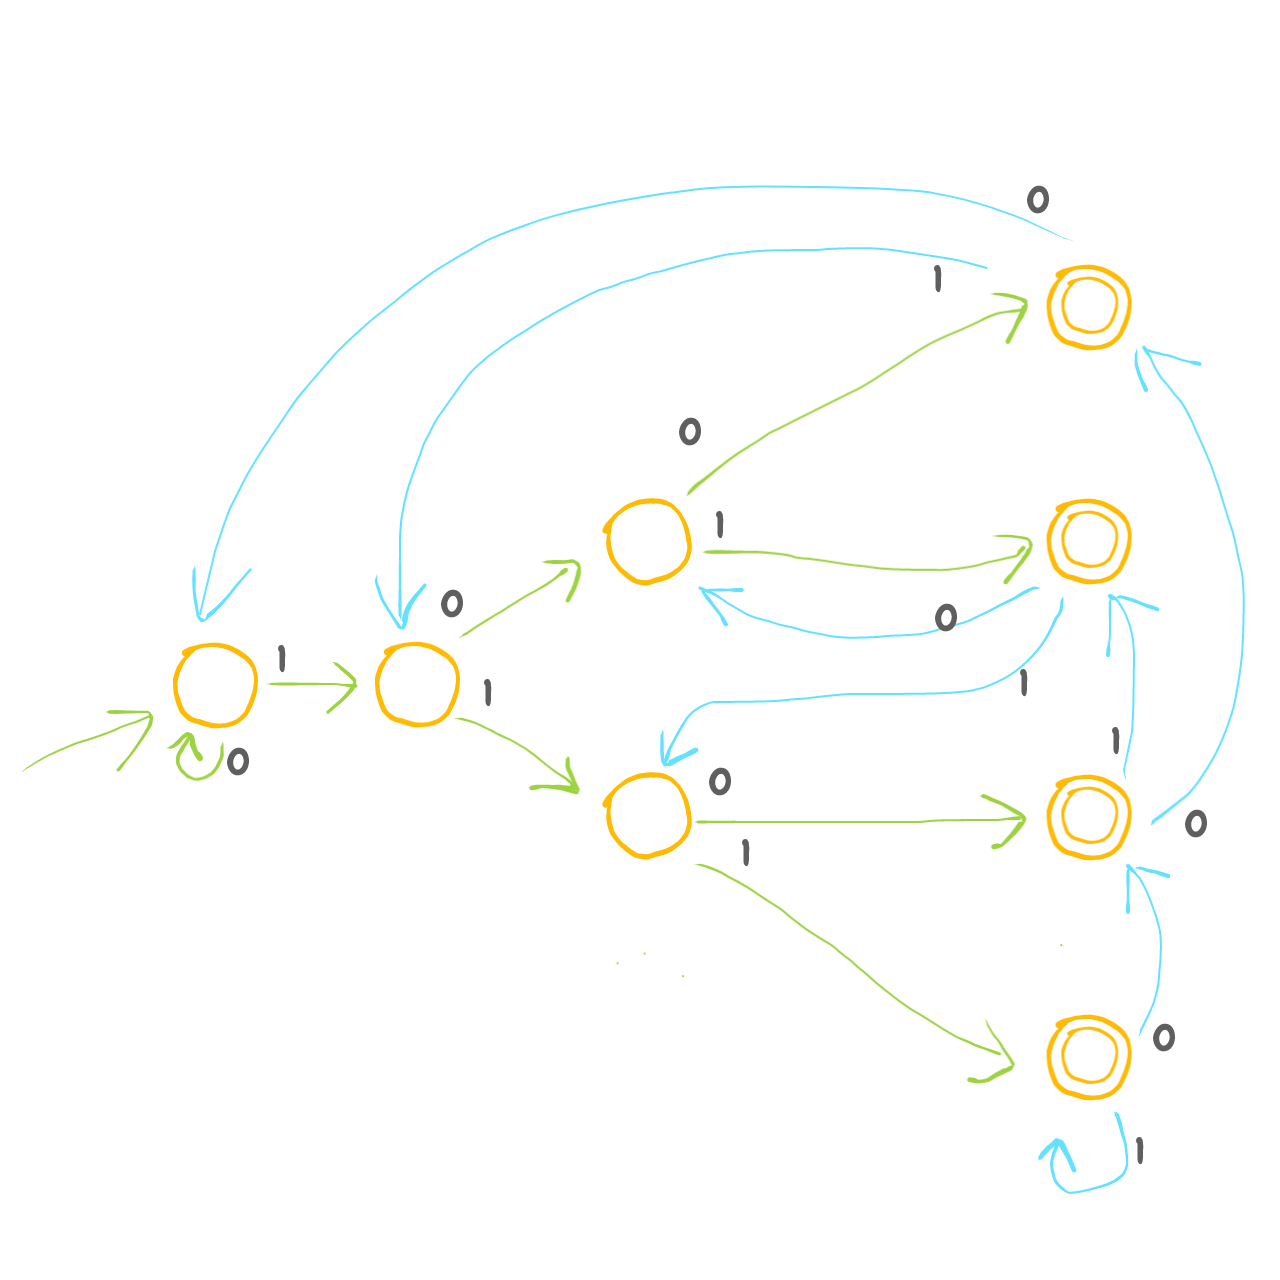
\includegraphics[scale=0.4]{data/2015-W-2.png}
    \caption{Question 2}
    \label{fig:w15-2}
\end{figure}



\paragraph{Question 3+4}
I'll prove that DFA that recognizes $L_n$:
\begin{equation*}
    L_n = \{ w\in \Sigma^* | \: |w| \geq 3  \text{ and n-th to the last letter of $w$ is $a$}\}
\end{equation*}
has no less than $2^n$ states. \textit{This is almost a copy-paste from \emph{Introduction to Automata Theory, Languages and Computation 3rd ed.}, Chapter 2.3.6}.

Intuitively we need $2^n$ states to remember every possible ending of length $n$: we can encode it as a binary string of length $n$.
Now, I'll show that there's no such DFA with less than $2^n$ states.

Suppose that there's DFA $D$ recognizing $L_n$ with less tan $2^n$ states.
If so, then tere must exist a state $q$ in which $D$ is after reading two different sequences, say $x = x_1x_2\cdots x_n$ and $y = y_1y_2\cdots y_n$.
Since they are different, let $i\in N$ be the last position on which they differ.
By symmetry, assume that $x_i = a$ and $y_i = b$.
\begin{itemize}
    \item if $i = 1$, then $x = a\:x_2\cdots x_n$ and $y = b\:y_2\cdots y_n$.
    Which means that state $q$ is both accepting and non-accepting.
    \item if $i > 1$, then we can append $(n-i)$ $b$'s to both $x$ and $y$. 
    Then a state $p$ in which $D$ is after reading $ax_{i+1}\cdots x_nb\cdots b$ and $by_{i+1}\cdots y_nb\cdots b$ is both accepting and non-accepting.
\end{itemize}
In both cases we get lead to contradiction.
Thus, DFA recognizing $L_n$ has at least $2^n$ states.

\begin{itemize}
    \item \textbf{Question 3:} Let $n = 3$. Then DFA recognizing $L_3$ has no less than $8$ states.
    \item \textbf{Question 4:} NFA recognizing $L_n$ has exactly $n+1$ states.
    Equivalent DFA has $2^n$ states.
\end{itemize}


\section{Problem 3 – Heap}
\paragraph{Question 1}
After inserting $21, 26$, the heap should look like:
\begin{verbatim}
        21
      /    \
    26      23
   /  \    /  \
 48   54  31   29
 |
 63
\end{verbatim}

\paragraph{Question 2}
After delete-min the heap should look like:
\begin{verbatim}
        25
      /    \
    48      42
   /  \
 35   73
\end{verbatim}

\paragraph{Question 3}
I understand \textit{visiting a node} by accessing an array in which heap is stored.

To insert a node, we first put it in fist available "slot" on the deepest level and then we "bubble" it up.
If the inserted element is smaller than other $n$ elements, then we'll traverse whole tree.
That means we will visit around $\lfloor log_2 (n+1)\rfloor$ elements.

\paragraph{Question 4}
First we, replace value with root with the last element in the heap array (and we erase that element).
Then, we need to "bubble down" this element.
At each iteration we'll visit its both children.
In worst case, we'll bubble it down to the deepest level.
So, we'll visit no more than $2 \lfloor log_2 (n-1) \rfloor$ elements.

\paragraph{Question 5}
Maximum element will reside somewhere on the deepest level, and we need to visit them all.
There are no more than $\lceil \frac{n}{2} \rceil$ elements on the deepest level.



\section{Problem 4 – Synchronization}

\paragraph{Question 1}
Suppose that there are two processes.
One of them may load value of \emph{queue\_head} before the other stores back incremented value.
Then, both processes will access the same buffer element, although they must not.

\paragraph{Question 2}
Semaphores (binary, counting), locks (test\&set, swap), monitors.


\paragraph{Question 3}
A semaphore is a shared variable with two defined operations executing atomically:
\emph{wait} and \emph{signal}.
\emph{wait()} decrements semaphore value, and if the value becomes less than zero, then process calling \emph{wait()} is made to sleep and is pushed to a queue.
\emph{signal()} increments semaphore value and, if the value is still negative, wakes up process at the beginning of the queue.

Note, that we only need to assure that every process is assigned different value of \emph{queue\_head}.
Initial setting:
\begin{verbatim}
Semaphore mutex = Semaphore(1);
\end{verbatim}
Code:
\begin{verbatim}
while(1) {
    wait(mutex);
    k = queue_head++;
    signal(mutex);
    ...
\end{verbatim}
